\chapter{Analyse de la demande et structuration de la réponse}

\section{Questionnaire pour le commanditaire}
Pour éviter de sélectionner un thème à partir de nos seules représentations, nous avons élaboré un questionnaire de recueil des besoins à destination de l'AFPA. Annoncé dès notre proposition du 9 septembre, il a été transmis en pièce jointe le 23 septembre 2026 après correction d'un premier envoi incomplet du 11 septembre.

Le document interrogeait notamment le public visé, son effectif, ses déplacements supposés, les situations de risque identifiées par le commanditaire, les attentes de l'établissement et les moyens matériels disponibles. Notre objectif était d'obtenir une première photographie du cadre de l'action, avant de la confronter aux caractéristiques effectives du public.

Mme LIÉGEOIS a renvoyé le questionnaire complété le 29 septembre, après un premier message du 28 septembre dans lequel la pièce jointe manquait. Le document renseigné a servi de support à notre rendez-vous du 1\textsuperscript{er} octobre.

\section{Réponses du commanditaire}
L'analyse du premier questionnaire a conduit à plusieurs décisions.
\begin{itemize}[leftmargin=*]
\item \textbf{Délimiter le public :} le projet, initialement ouvert à divers personnels et stagiaires, a été recentré sur une promotion de plomberie.
\item \textbf{Adapter l'effectif :} l'estimation initiale d'environ quarante personnes a été ramenée à une cible de dix à quinze, plus compatible avec les échanges et les manipulations en petits groupes.
\item \textbf{Vérifier les mobilités :} les modes de déplacement évoqués par le commanditaire concernaient l'établissement de manière générale et ne décrivaient pas nécessairement la promotion ciblée.
\item \textbf{Hiérarchiser les risques :} l'alcool, le téléphone, les stupéfiants, les médicaments et la banalisation des risques ont été évoqués comme pistes, sans que leur prévalence réelle soit établie.
\item \textbf{Identifier les contraintes :} l'action était envisagée dans les locaux du centre, avec des moyens de projection et un espace extérieur potentiellement mobilisable.
\end{itemize}

La réponse du commanditaire a donc fourni un \textbf{cadrage} utile, mais non un diagnostic suffisant. En particulier, les comportements attribués de manière générale à certains stagiaires de l'AFPA ne devaient pas être extrapolés à la nouvelle promotion.

\section{Questionnaire aux participants}
Nous avons conçu un second questionnaire anonyme destiné aux stagiaires de plomberie. Il comporte trente questions réparties en huit domaines : situation de déplacement ; vitesse ; téléphone et distracteurs ; alcool ; stupéfiants ; médicaments ; ceinture ; perception globale des risques.

Le choix de ces rubriques répondait à trois objectifs : établir quelques connaissances de base, recueillir des comportements déclarés et rechercher les représentations pouvant influencer les décisions. Plusieurs scénarios s'inscrivent dans l'univers professionnel du plombier : retard sur un chantier, appel d'un client, fin de journée ou déplacement en véhicule utilitaire.

Le questionnaire a été adressé à Mme LIÉGEOIS le \textbf{26 octobre 2026 à 11\,h\,49}. Elle a répondu le jour même qu'elle le ferait compléter dans la semaine. Nous avons effectué une relance le 29 octobre ; Mme LIÉGEOIS a indiqué qu'elle transmettrait les formulaires numérisés. Notre analyse repose finalement sur \textbf{treize réponses exploitables}, regroupées dans un fichier de données.

L'anonymat était annoncé aux stagiaires : aucune identité n'était demandée. Les réponses sont exploitées collectivement et ne servent ni à qualifier une personne ni à établir une infraction. Les questions relatives aux comportements reposent sur l'auto-déclaration, susceptible de biais de mémoire et de désirabilité sociale.

\section{Synthèse des réponses des participants}
\subsection{Méthode de traitement}
Nous avons rapproché les réponses individuelles des questions posées, puis compté les effectifs de réponses correctes, erronées ou révélatrices d'un risque. Le dénominateur utilisé est de treize répondants. Certaines questions, malgré leur formulation au singulier, ont accepté plusieurs réponses dans le formulaire numérique. Nous le signalons lorsque cela influe sur la lecture des résultats.

La distinction entre \emph{connaissances / perceptions} et \emph{comportements / intentions déclarés} est essentielle : une connaissance erronée n'est pas un comportement observé, et une intention ne constitue pas une preuve d'action réelle.

\subsection{Profil de déplacement du groupe}
\begin{itemize}[leftmargin=*]
\item \textbf{11/13} répondants déclarent posséder le permis B.
\item \textbf{2/13} ne le possèdent pas. 
\item \textbf{4/13} déclarent conduire tous les jours.
\item \textbf{2/13} plusieurs fois par semaine.
\item \textbf{4/13} occasionnellement.
\item \textbf{3/13} jamais. 

\end{itemize}

Ces résultats confirment que le groupe n'est pas homogène en matière d'expérience de conduite. Les situations pédagogiques doivent donc rester accessibles à tous les usagers, conducteurs actuels ou futurs.

\subsection{L'alcool : un besoin prioritaire en connaissances et en perception}
La figure~\ref{fig:diagnostic-afpa} met en évidence, pour l'alcool, le taux le plus élevé de \emph{signaux de besoin en connaissances et en perception} parmi les six thèmes étudiés : \textbf{69,23\,\% (9/13)}. Le volet \emph{comportements et situations à risque} atteint \textbf{53,85\,\% (7/13)}. Ces valeurs, issues de l'indicateur synthétique présenté sur la figure, montrent l'intérêt d'une sensibilisation sur cette problématique, sans constituer à elles seules une mesure d'alcoolémie ni une observation directe des conduites.

\begin{table}[htbp]
\centering\small
\caption{Indicateurs de synthèse de la figure~\ref{fig:diagnostic-afpa} : alcool (13 répondants)}
\begin{tabularx}{\textwidth}{@{}Xrr@{}}
\toprule
\rowcolor{bleuECSR}
\textcolor{white}{\textbf{Catégorie de signaux}} & \textcolor{white}{\textbf{Effectif affiché}} & \textcolor{white}{\textbf{Taux affiché}} \\
\midrule
Connaissances / perception & 9/13 & 69,23\,\% \\
Comportements / situations à risque & 7/13 & 53,85\,\% \\
\bottomrule
\end{tabularx}
\end{table}

Ces constats figurent dans notre diagnostic commun. Toutefois, afin d'approfondir chaque thème sans redondance, \textbf{l'analyse détaillée des réponses sur l'alcool et la réponse pédagogique correspondante seront développées dans le mémoire de ma collègue Manane SADIK}. Le présent mémoire se concentre sur les distracteurs, notamment sur les sollicitations téléphoniques pendant les déplacements professionnels des futurs plombiers.

\subsection{Le téléphone et les distracteurs : un besoin principalement comportemental}
Pour le téléphone et les distracteurs, la figure~\ref{fig:diagnostic-afpa} indique \textbf{38,46\,\% (5/13)} de signaux de besoin en \emph{connaissances et perception}, contre \textbf{61,54\,\% (8/13)} pour les \emph{comportements et situations à risque}. Ce dernier taux est le \textbf{plus élevé des six thèmes} dans la catégorie comportementale. Il dépasse celui de l'alcool (53,85\,\%, soit 7/13) et ceux de la vitesse ou des stupéfiants (38,46\,\%, soit 5/13 chacun).

\begin{table}[htbp]
\centering\small
\caption{Indicateurs de synthèse de la figure~\ref{fig:diagnostic-afpa} : téléphone et distracteurs (13 répondants)}
\begin{tabularx}{\textwidth}{@{}Xrr@{}}
\toprule
\rowcolor{bleuECSR}
\textcolor{white}{\textbf{Catégorie de signaux}} & \textcolor{white}{\textbf{Effectif affiché}} & \textcolor{white}{\textbf{Taux affiché}} \\
\midrule
Connaissances / perception & 5/13 & 38,46\,\% \\
Comportements / situations à risque & 8/13 & 61,54\,\% \\
\bottomrule
\end{tabularx}
\end{table}

Les questions individuelles apportent un éclairage complémentaire : \textbf{8/13} stagiaires déclarent consulter une notification ou un message au volant au moins occasionnellement (Q11), tandis que \textbf{11/13} savent que l'usage d'un dispositif mains libres ne supprime pas totalement le risque de distraction (Q10). Ces effectifs correspondent à des questions précises et \emph{ne doivent pas être confondus} avec les deux indicateurs synthétiques du graphique. Le contraste entre les connaissances et les comportements déclarés oriente notre démarche : \textbf{la connaissance d'un danger n'entraîne pas nécessairement une décision protectrice}.

Dans le métier de plombier, ce décalage peut se manifester lors d'un appel du client, d'une demande du responsable ou d'une recherche d'adresse en cours de déplacement. Ces situations justifient une approche pédagogique fondée sur l'expérience de la double tâche et sur la recherche de réponses professionnelles adaptées.

\subsection{Comparaison des six thématiques et limites de l'analyse}
La figure~\ref{fig:diagnostic-afpa} présente deux catégories de signaux pour chacun des six thèmes. Les valeurs sont reproduites ci-dessous, sans les assimiler à des taux d'accidents ni à des infractions constatées.

\begin{table}[htbp]
\centering\small
\caption{Lecture chiffrée de la figure~\ref{fig:diagnostic-afpa} (n = 13)}
\begin{tabularx}{\textwidth}{@{}Xrr@{}}
\toprule
\rowcolor{bleuECSR}
\textcolor{white}{\textbf{Thème}} & \textcolor{white}{\textbf{Connaissances / perception}} & \textcolor{white}{\textbf{Comportements / situations à risque}} \\
\midrule
Alcool & 69,23\,\% (9/13) & 53,85\,\% (7/13) \\
Téléphone / distracteurs & 38,46\,\% (5/13) & 61,54\,\% (8/13) \\
Vitesse & 38,46\,\% (5/13) & 38,46\,\% (5/13) \\
Médicaments & 38,46\,\% (5/13) & 23,08\,\% (3/13) \\
Stupéfiants & 15,38\,\% (2/13) & 38,46\,\% (5/13) \\
Ceinture de sécurité & 30,77\,\% (4/13) & 15,38\,\% (2/13) \\
\bottomrule
\end{tabularx}
\end{table}

\begin{figure}[htbp]
\centering
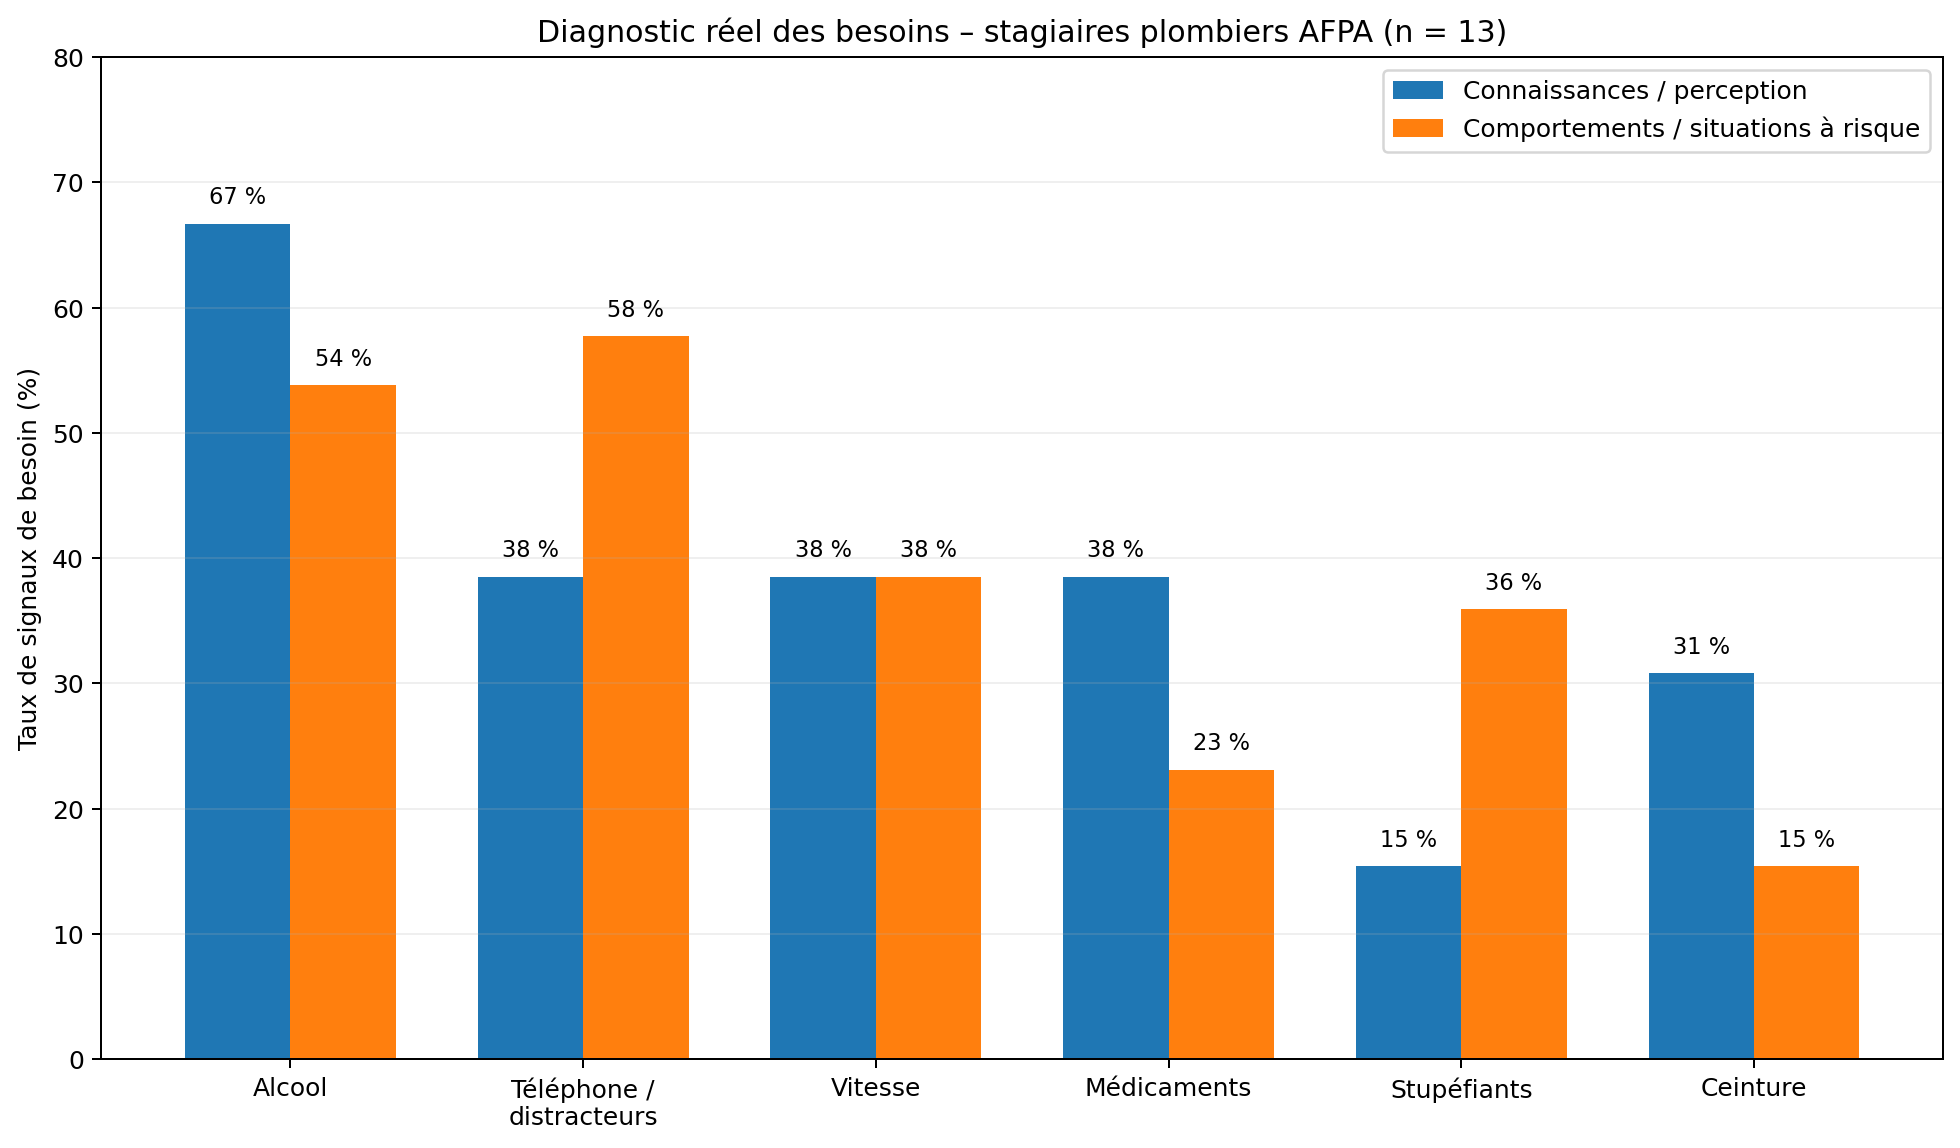
\includegraphics[width=\textwidth]{images/diagnostic_afpa_13_repondants.png}
\caption{Signaux de besoin en sécurité routière par thème, selon deux catégories d'analyse (13 répondants).}
\label{fig:diagnostic-afpa}
\end{figure}

La comparaison fait apparaître deux profils : l'alcool occupe la première place pour les connaissances et perceptions (69,23\,\%), tandis que le téléphone et les distracteurs arrivent en tête pour les comportements et situations à risque (61,54\,\%). La vitesse, les médicaments, les stupéfiants et la ceinture de sécurité présentent aussi des signaux de besoin, mais aucun ne dépasse ces deux maxima dans les catégories respectives.

\textbf{Précaution méthodologique :} la figure affiche des effectifs et des pourcentages de synthèse ; elle ne détaille pas ici les règles de construction de chaque indicateur à partir des questions du formulaire. Les valeurs sont donc présentées comme des \emph{signaux descriptifs}, et non comme le nombre de personnes ayant commis une infraction. Avec seulement treize répondants et des données déclaratives, cette analyse éclaire les choix pédagogiques pour ce groupe sans permettre de généralisation à l'ensemble de l'AFPA ou des professionnels de la plomberie. Les questions autorisant plusieurs sélections appellent la même prudence.

\section{Objectif proposé au commanditaire}
\subsection{Objectifs opérationnels du scénario « distracteurs »}
L'objectif général envisagé est d'\emph{amener les stagiaires plombiers à reconnaître les distracteurs pendant un déplacement professionnel, à expérimenter leurs effets sur l'attention et à adopter une organisation sûre face aux sollicitations}. À l'issue de la séance, chaque participant devrait pouvoir :
\begin{enumerate}[leftmargin=*]
\item citer et illustrer les quatre dimensions de la distraction : visuelle, manuelle, auditive et cognitive ;
\item expliquer, à partir d'un exemple de distance parcourue et des exercices réalisés, pourquoi quelques secondes d'inattention peuvent être dangereuses ;
\item repérer au moins deux effets d'une double tâche sur la trajectoire, le respect des consignes ou la réaction à un signal simple ;
\item identifier les risques et les pressions d'un appel ou d'un message professionnel en cours de trajet ;
\item proposer une conduite protectrice : préparer son GPS, laisser sonner, trouver un lieu de stationnement approprié, s'arrêter puis répondre.
\end{enumerate}

Ces objectifs pourront être évalués par questionnement, observation des exercices, restitution collective et quiz final. Un participant non conducteur pourra mobiliser les mêmes compétences comme futur conducteur ou usager de la route.

\section{Lettre de mission et note de cadrage}
À ce stade, les accords et les contraintes sont documentés principalement par les courriels échangés avec Mme LIÉGEOIS : intervention gratuite proposée par notre binôme, public cible de stagiaires plombiers, effectif envisagé de dix à quinze, durée d'environ deux heures et date du 4 décembre 2026 au matin. Le questionnaire commanditaire et l'entretien du 1\textsuperscript{er} octobre complètent ce cadrage.

Nous ne présentons pas ces échanges comme une lettre de mission formellement signée. Une note de cadrage reprenant les objectifs, rôles, besoins matériels, conditions d'accueil et modalités d'évaluation est proposée en annexe. Elle restera à valider avec les personnes concernées si nécessaire.

\section{Outils et méthodes utilisés}
Notre stratégie pédagogique combine la méthode interrogative, des apports courts, des supports visuels, l'observation de vidéos d'attention sélective, une démonstration comparative en extérieur et un débriefing collectif. L'objectif est de faire émerger l'écart entre \emph{se croire attentif} et \emph{disposer réellement de toutes ses ressources attentionnelles}.

Le nouveau support « Smartphone au volant : le piège des chantiers » présente le contexte professionnel, les quatre formes de distraction, des exercices d'attention sélective et de cécité attentionnelle, des ordres de grandeur de distance parcourue, la réglementation et les gestes de prévention. Sa version PDF du 13 novembre 2026 comporte trente pages ; les séquences documentées portent sur les situations de chantier, les types de distraction, deux vidéos (comptage de ballons et de passes), des données ONISR, les distances parcourues, l'article R.412-6-1, les sanctions, les réflexes préventifs et un quiz final. L'activité pédestre extérieure est une séquence complémentaire décrite dans notre protocole et dans le tableau synoptique. Le parcours pédestre « Même parcours, attention différente » prolonge ces apports par une expérience comparée sans véhicule.

La première proposition de séance « Sur la route du chantier --- Alcool et distracteurs » reste une trace de l'évolution de notre conception : elle présentait une valise dose bar, une activité SAM et différents jeux de rôle. Ces outils ne doivent pas être décrits comme réalisés ni comme nécessairement conservés dans le scénario recentré sur les distracteurs.

\subsection{Recherche de partenaires et de matériel}
La Préfecture des Alpes-Maritimes met à notre disposition une valise « dose bar », une « tête de Sam », des éthylotests, des affiches, des flyers et des goodies. Ce prêt, encadré par une convention signée, prévoit un retrait le 27 novembre 2026 et une restitution le 7 décembre 2026.

\section{Cahier des charges}
\begin{longtable}{@{}p{0.29\textwidth}p{0.64\textwidth}@{}}
\toprule
\rowcolor{bleuECSR}
\textcolor{white}{\textbf{Élément}} & \textcolor{white}{\textbf{Cadrage retenu ou point à confirmer}} \\
\midrule
\endfirsthead
\toprule
\rowcolor{bleuECSR}
\textcolor{white}{\textbf{Élément}} & \textcolor{white}{\textbf{Cadrage retenu ou point à confirmer}} \\ \midrule
\endhead
Commanditaire & AFPA Nice, interlocutrice : Mme Muriel LIÉGEOIS. \\
Intervenants & Sam FOKAM WABO et Manane SADIK, stagiaires TP ECSR, en co-animation. \\
Public & Promotion de stagiaires plombiers ; treize répondants au diagnostic ; effectif du jour à relever. \\
Date et horaire & 4 décembre 2026 au matin ; horaire exact à confirmer. \\
Durée & Environ deux heures, à répartir entre accueil, apports, activités et bilan. \\
Lieu & AFPA Nice ; salle de formation et parcours pédestre extérieur, sous réserve d’autorisation et de reconnaissance préalable du terrain. \\
Objectif général & Reconnaître les distracteurs et décider comment gérer sans risque les sollicitations professionnelles ; scénario récent à confirmer avec le commanditaire. \\
Méthodes & Interrogative, participative, visionnage guidé, expérimentation pédestre, observation comparée et débriefing. \\
Moyens & Vidéoprojecteur, tableau, supports de séance et matériels de prévention ; inventaire final à confirmer ; convention signée par la directrice de cabinet transmise le 10 novembre, retrait prévu le 27 novembre et restitution le 7 décembre au matin. \\
Sécurité & Aucun véhicule en mouvement ni consommation d’alcool ; parcours exclusivement à pied, aire isolée et dégagée, consignes de non-collision, balle souple sans visée du visage, possibilité de refuser une tâche. \\
Évaluation & Questions de vérification, mises en situation, questionnaire de satisfaction et retour commanditaire à recueillir. \\
Traçabilité & Questionnaires anonymisés, échanges, convention, supports, tableau synoptique et bilan de séance. \\
\bottomrule
\end{longtable}

\section{Tableau synoptique}
Le tableau synoptique ci-après reprend les \textbf{six colonnes du modèle fourni} : séquences, objectif, durée, contenu, méthodes/techniques et moyen. Afin de conserver ces rubriques sans réduire excessivement la lisibilité, \textbf{seule la page du tableau} est présentée au format paysage. Il s'agit d'une \emph{préparation} de deux heures, susceptible d'être ajustée selon les conditions de l'intervention du 4 décembre 2026.

\clearpage
\newgeometry{left=0.8cm,right=0.8cm,top=1.2cm,bottom=1.2cm}
\begin{landscape}
\thispagestyle{plain}
\begin{center}
{\Large\bfseries Tableau synoptique prévisionnel -- Sensibilisation aux distracteurs}\\[2pt]
{\small AFPA Nice -- stagiaires plombiers -- co-animation -- durée totale : 120 minutes}
\end{center}
\vspace{1mm}
\begingroup
\scriptsize
\setlength{\arrayrulewidth}{0.4pt}
\renewcommand{\arraystretch}{1.05}
\setlength{\tabcolsep}{2pt}
%\begin{adjustbox}{max totalsize={\linewidth}{0.90\textheight},center}
\begin{adjustbox}{width=\linewidth,center}
%\begin{tabular}{@{}p{2.9cm}p{4.0cm}p{1.4cm}p{6.0cm}p{4.1cm}p{3.8cm}@{}}
\begin{tabular}{@{}p{3.2cm}p{4.4cm}p{1.5cm}p{6.8cm}p{4.6cm}p{4.3cm}@{}}
%\begin{tabular}{|p{3.2cm}|p{4.4cm}|p{1.5cm}|p{6.8cm}|p{4.6cm}|p{4.3cm}|}
\toprule
\rowcolor{bleuECSR}
\textcolor{white}{\textbf{Séquences}} & \textcolor{white}{\textbf{Objectif}} & \textcolor{white}{\textbf{Durée}} & \textcolor{white}{\textbf{Contenu}} & \textcolor{white}{\textbf{Méthodes/Techniques}} & \textcolor{white}{\textbf{Moyen}} \\
\midrule
% Coloration explicite de chaque ligne : stable avec booktabs et adjustbox.
\rowcolor{orangeECSR!18}
Présentation / accueil & Identifier les attentes et installer un climat de confiance. & 8 min & Présentation des intervenants ; métier de plombier, déplacements et attentes des participants. & Tour de table bref ; questionnement oral. & Diaporama, vidéoprojecteur, tableau. \\
\midrule
Question d'ouverture & Susciter l'intérêt et faire émerger la problématique. & 2 min & « Un appel client urgent justifie-t-il de répondre immédiatement au volant ? » & Question d'accroche ; débat flash. & Diapositive, tableau. \\
\midrule
\rowcolor{orangeECSR!18}
Évaluation initiale & Repérer les représentations et connaissances de départ. & 6 min & Reconnaissance des distracteurs ; risques du mains-libres ; réaction à un SMS professionnel. & Questions diagnostiques ; vote / échanges ; sans jugement. & Questions projetées, tableau, feutres. \\
\midrule
Annonce des objectifs & Faire comprendre les acquis recherchés. & 4 min & Identifier les distractions ; observer l'effet de la double tâche ; choisir une réponse sûre face aux sollicitations. & Présentation interrogative ; reformulation. & Diaporama, tableau. \\
\midrule
\rowcolor{orangeECSR!18}
Cours : types de distraction & Distinguer les quatre formes de distraction. & 13 min & Distractions visuelle, manuelle, auditive et cognitive ; exemples d'appel, SMS, GPS, recherche d'adresse. & Exposé dialogué ; exemples métier. & Diaporama, vidéoprojecteur. \\
\midrule
Mise en évidence de l'attention & Constater les limites de l'attention sélective. & 12 min & Vidéo(s) d'observation ; repérage d'éléments inattendus ; comparaison des perceptions. & Observation individuelle ; débat / débriefing. & Vidéo préchargée, ordinateur, écran ; variante orale. \\
\midrule
\rowcolor{orangeECSR!18}
Cours : risques et règles & Relier la distraction aux conséquences routières et au droit. & 15 min & Distance parcourue sans regarder la route ; risque de collision ; interdictions et sanctions du téléphone tenu en main. & Exposé interactif ; calcul simple ; questions. & Diaporama, tableau, sources réglementaires. \\
\midrule
Réflexes professionnels & Savoir gérer un appel ou message pendant un trajet. & 8 min & Anticiper les communications ; laisser sonner ; stationner dans un lieu sûr ; rappeler à l'arrêt. & Étude de cas « client / chef de chantier » ; échange. & Diaporama, fiche scénario. \\
\midrule
\rowcolor{orangeECSR!18}
Préparation extérieure & Connaître les consignes et les critères d'observation. & 8 min & Présentation du parcours pédestre ; volontaires, observateurs, sécurité ; temps, erreurs, hésitations. & Démonstration ; répartition des rôles. & 4--5 plots, objets, téléphone factice, fiches, chronomètre. \\
\midrule
Opérationnalisation : parcours & Expérimenter la double tâche et observer ses effets. & 32 min & Même parcours sans distracteur, puis appel, SMS, événement visuel avec balle souple, sollicitations cumulées (si réalisable). & Expérimentation à pied ; observation comparée ; rotations ciblées de volontaires. & Plots, téléphone, SMS préparés, balle en mousse, chronomètre, grille. \\
\midrule
\rowcolor{orangeECSR!18}
Débriefing / transfert & Identifier les écarts et transposer à la conduite d'un utilitaire. & 8 min & Comparaison des temps, erreurs et réactions ; place des pressions professionnelles ; stratégies de prévention. & Analyse collective ; mise en commun des observations. & Grille d'observation, tableau, feutres. \\
\midrule
Bilan final / évaluation & Vérifier les acquis et fixer une conduite à tenir. & 4 min & Questions de contrôle ; reformulation du réflexe « s'arrêter avant de répondre » ; conclusion et remerciements. & Évaluation orale flash ; synthèse. & Questions de bilan, tableau. \\
\midrule
\rowcolor{bleuECSR}\textcolor{white}{\textbf{TOTAL}} & \textcolor{white}{\textbf{Séance prévisionnelle (intérieur et extérieur).}} & \textcolor{white}{\textbf{120 min}} & \multicolumn{3}{>{\columncolor{bleuECSR}}l}{\textcolor{white}{\textit{Temps indicatifs, à ajuster après observation de l\'action réelle.}}} \\
\bottomrule
\end{tabular}
\end{adjustbox}
\endgroup
\end{landscape}
\restoregeometry
\clearpage

\paragraph{Contraintes de faisabilité.}
Quinze stagiaires sont envisagés, mais il ne serait pas réaliste de leur faire réaliser individuellement les cinq passages dans une enveloppe de 35 minutes. L'atelier repose donc sur \textbf{quelques volontaires avec observation active du reste du groupe} : les observateurs notent les indicateurs, comparent les essais et participent au débriefing. Les passages sont adaptables selon l'effectif présent et les conditions matérielles. Aucun résultat ne sera annoncé d'avance : le chronométrage et les erreurs seront relevés sur place.

\paragraph{Vigilance documentaire.}
Le diaporama contient des chiffres d'accidentalité, des pourcentages et des sanctions qui devront être contrôlés dans leurs sources officielles et situés à leur bonne date avant l'animation. Les vidéos ne peuvent être utilisées que si leur diffusion est autorisée et si le matériel de projection fonctionne ; une variante orale de l'exercice devra être prévue.
